\documentclass[letterpaper, openright, 11pt]{article}
\usepackage[utf8]{inputenc}
\usepackage[english]{babel}
\usepackage{graphicx}
\usepackage{amsmath}
\usepackage{amssymb}
\usepackage{amsfonts}
\usepackage{anysize}
\marginsize{2cm}{2cm}{2cm}{2cm}
\usepackage{fancyhdr}
\setlength{\headheight}{15pt}
\usepackage{multicol}
\usepackage{float}
\usepackage{hyperref}

\begin{document}

\lhead{Nantrobot}
\rhead{joy\_controller}

\begin{center}

\begin{figure}[H]
	\centering
	
\includegraphics[scale=0.15]{Nantrobot1.JPG}
\end{figure}
\noindent\makebox[\linewidth]{\rule{\paperwidth}{0.4pt}}

\Large Package\\
\LARGE Joy\_Controller\\

\noindent\makebox[\linewidth]{\rule{\paperwidth}{0.4pt}}

\end{center}

The following package was created by the team \textbf{Nantrobot} of the \textit{École Centrale de Nantes} to provide an easier testing hardware-software tool for future competitions and developments. It requires
\begin{itemize}
\item ROS
\item package Joy
\item package Geometry\_msgs
\item Thrustmaster Controller or equivalent
\end{itemize} 

\section{Introduction}

During a robot development there are many routines, programs, and sensors to test. Therefore if we want to test them we would have to change the code, load it into the robot and restart it. The purpose of the package is to control the robot's direction, publish the controller's buttons and sticks, if the controller is on and some states for testing. Then with the states it's possible to switch these routines in real-time to make testing faster for developers and with the buttons to specific tasks. 

\section{Controller conventions}

\begin{figure}[H]
	\centering
	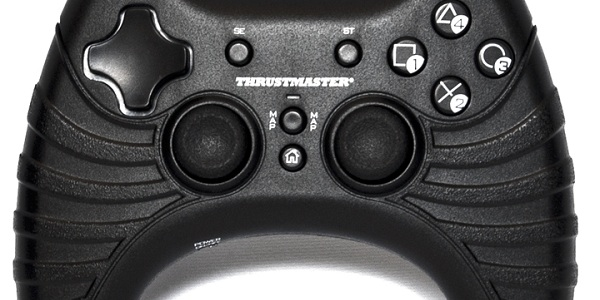
\includegraphics[scale=0.6]{cont-front.jpg}
	\caption{Controller front}
\end{figure}

\begin{figure}[H]
	\centering
	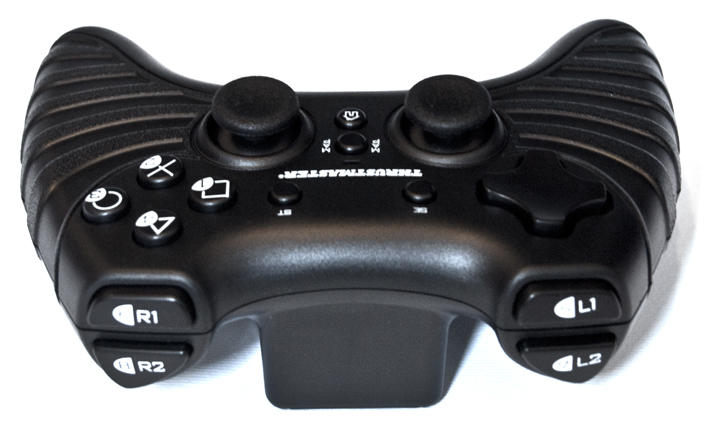
\includegraphics[scale=0.4]{cont-back.jpg}
	\caption{Controller back}
\end{figure}
We will name the controller components as follows:
\begin{multicols}{4}
\begin{enumerate}
\item square
\item cross
\item circle
\item triangle
\item L1
\item R1
\item L2
\item R2
\item SE
\item ST
\item Stick 1 pressed
\item Stick 2 pressed
\end{enumerate}
\end{multicols}
The left Stick will be called \textbf{Stick 1} and the right stick \textbf{Stick 2}. The home button will serve as \textbf{on\_state} for the controller and the pad will be the third stick but only with int values (\textbf{IntStick}).

\pagestyle{fancy}

\section{Message managment}

We'll have two messages published:
\begin{center}
\begin{multicols}{2}
\noindent \Large geometry\_msgs/Point Message\\
\normalsize As \textbf{PointCons}\\
This will be used to command the robot using the axes $X$ and $Y$ as for \textit{Vertical} with the Stick 1 and \textit{Horizontal} with the Stick 2.\\
\Large joy\_controller/joystick Message\\
\normalsize As \textbf{JoyStick}\\
This will be used for publishing the states and the values of each component.
\end{multicols}
\end{center}

\section{Using the controller}

Now that we have our messages defined let's make some remarks:
\begin{itemize}
\item If the on\_state is Off (0) then no change  will be reflected on the values. Then if you press the cross and switch the controller off the cross will remain pressed. The States will remain the same as well. But for security reasons the \textit{PointCons} values will always be reset so that the robot doesn't collide.
\item The Stick 1 can only control the vertical axis (y) of \textit{PointCons}.
\item The Stick 2 can only control the horizontal axis (x) of \textit{PointCons}.
\item There two states:
\begin{tabbing}
\hspace{4cm}\=\hspace{4cm}\=\kill
 State 1 \> State 2 \> Value \\ 
 Square \> L1 \> 1\\
 Cross \> R1 \> 2\\ 
 Circle \>  L2 \> 3\\ 
 Triangle \> R2 \> 4
\end{tabbing} 
And their prupose is to serve testing.
\end{itemize}

\section{Final Remarks}

The \textit{launch File} is configured to use the sensor $"/dev/input/js1"$ and it can be changed easily if required. The meaning of the states are completely up to the developer. 

\section{Contact}

Any problem, improvements, suggestions to\\
\textit{dpalmac@dcc.uchile.cl}\\
and\\
\textit{alexis.martin.2@eleves.ec-nantes.fr}.

\end{document}